\section{Evaluation}\label{sec:evaluation}

% This section shows benchmark designs and results of each papers' implementation by us.
% sand and fusionize attempt to solve similar problems -> same evaluation and
% comparison: latency benchmark aimed at measuring network overheads
% profaastinate is different -> own evaluation:
% all evaluations' results are discussed together in section
% \ref{sec:discussion}

This section provides an overview of our benchmark designs and the results of
our implementation for each paper. SAND and \textsc{Fusionize} attempt to solve
similar problems, hence they share the same evaluation and are directly compared
to each other. We primarily focus on the latency benchmark designed to measure
network overheads. On the other hand, \textsc{ProFaaStinate} is different from
the other approaches and therefore requires its own specific evaluation. The
outcomes of all these evaluations will be collectively discussed in Section
\ref{sec:discussion}.

\subsection{Fusionize and SAND}

% for fusionize and sand we designed a benchmark aimed at isolating the network
% overhead to simulate cascading cold starts and double billing. We chose method
% best showcases end to end latencies between faas functions we decided for
% synthetic base load to investigate system's performance under maximum stress.

% To showcase maximum latency, we designed two tasks, shown in Figure X,
% \emph{interface} task and \emph{counter} task. The counter Task receives a
% number and returns the number, incremented by one. The interface task receives
% a \emph{destination} number by the user and invokes the counter task, starting
% with the number zero. The result of the counter task is then used to invoke
% the counter task again until the destination number is reached.

% This proposed load generator is unconventional, as it resides within the
% system under test. However, this design allows for function invocation within
% the platfrom and most importantly \emph{between} functions. To start the
% benchmark, only the interface task needs to be invoked with destination
% number and latency between invocation and result is to measured.

\subsubsection{Experiment Setup}
\label{subsubsec:evaluation:fusionize_and_sand:experiment_setup}

For \textsc{Fusionize} and SAND, we have constructed a benchmark with the
intention of isolating networking overhead. This is designed to simulate scenarios
involving cascading cold starts and double billing. We made this decision based
on our belief that this approach most effectively displays the end-to-end
latencies that can occur between FaaS functions. We chose to employ a synthetic
base load for our testing in order to examine the system's performance under
maximum stress.

In order to illustrate the maximum latency, we devised two tasks. These tasks,
which can be seen in Figure \ref{fig:bench}, are known as the \emph{interface}
and \emph{counter} tasks. The objective of the counter task is to receive a
number and return the same number after it has been increased by one. The
interface task works by accepting a \emph{destination} number supplied by the
user, then invoking the counter task, beginning with the number zero. Following
this, the result of the counter task is used to again invoke the counter task,
repeating until the destination number is reached.

Our proposed load generator has an unconventional design, as it resides within
the system under test (SUT). However, this design allows function invocation
within the platform, and, even more crucially, between functions. This is
important, as both Fusionize and SAND are revolving around the communication
between FaaS functions. To initiate the benchmark, only the interface task needs
to be invoked with the destination number. The latency between the invocation
and result must then be measured.

% - In a production setting, Nuclio is run in k8s cluster
% - We configured deployment of our approaches for k8s
% - For our benchmarks we deployed our system in local Minikube cluster

In a production environment, Nuclio operates within a k8s cluster. We have
successfully configured the deployment of our approaches for operation within
the k8s environments. For benchmarking purposes, we deployed our system within a
local Minikube\footnote{\url{https://minikube.sigs.k8s.io/}} cluster.

\begin{figure}
    \centering
    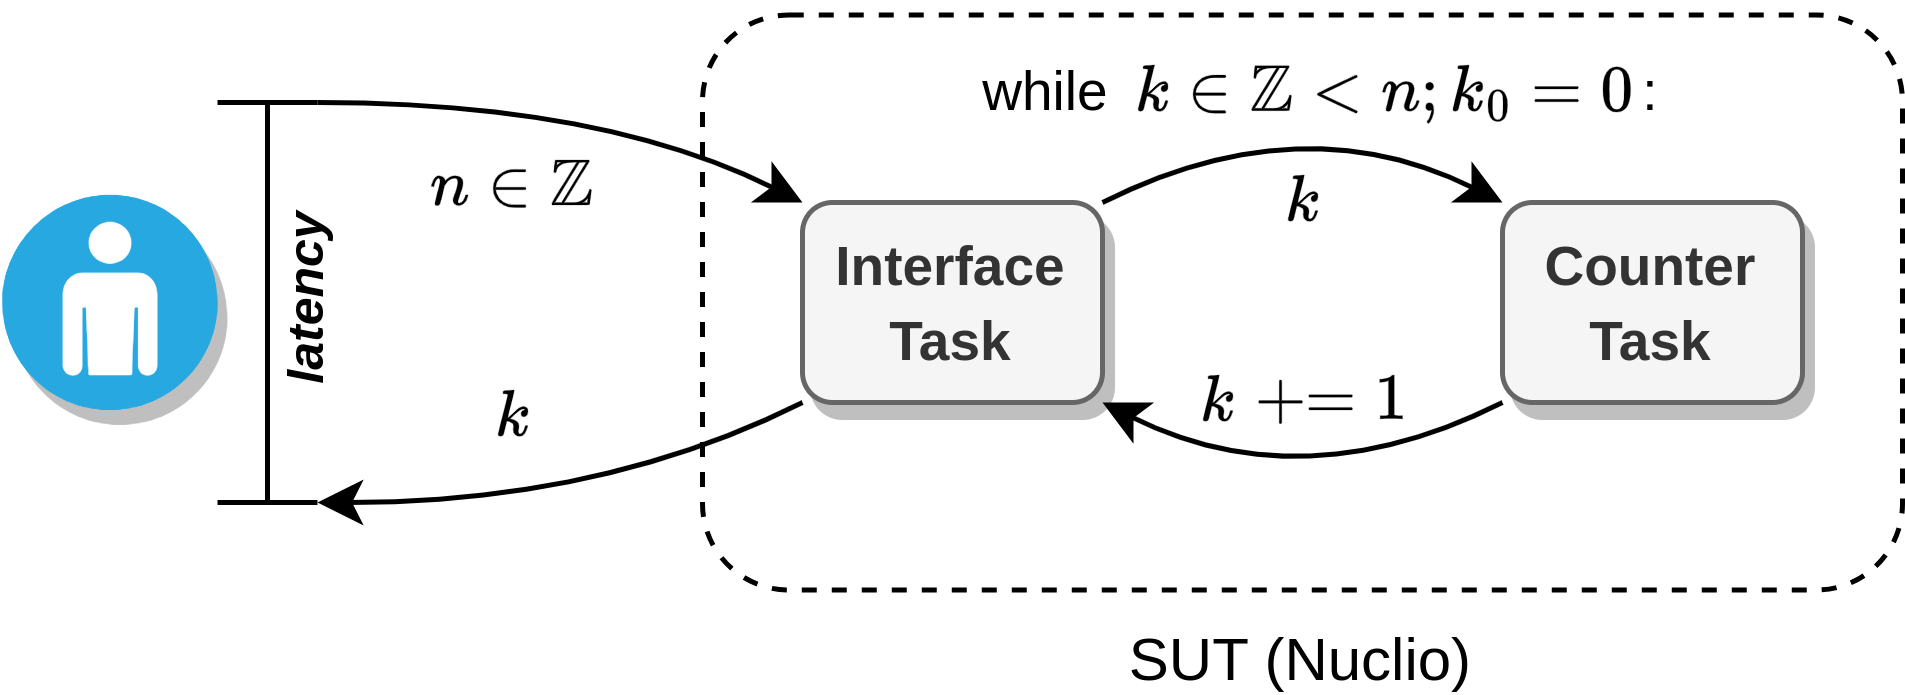
\includegraphics[width=\linewidth]{figures/bench}
    \caption{
        The Counter Task increments a given number by one. The Interface Task
        receives a target number from the user and repeatedly invokes the
        Counter Task, starting at zero, until the target number is achieved. The
        Interface Task then returns this number to the user upon completion of
        the benchmark run. This allows the user to measure the total end-to-end
        latency.
    }
    \label{fig:bench}
\end{figure}

\subsubsection{Results}
\label{subsubsec:evaluation:fusionize_and_sand:results}

\begin{figure}
    \centering
    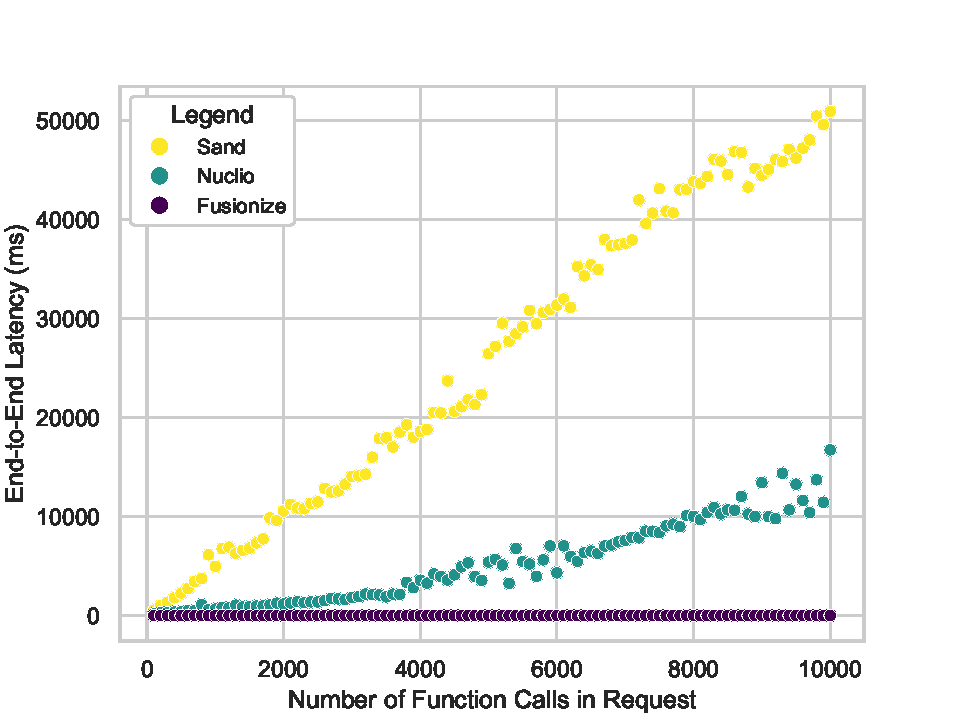
\includegraphics[width=\linewidth]{figures/latency_sand_fusionize}
    \caption{
        Results of our benchmark outlined in Figure \ref{fig:bench}. Our SAND
        implementation increases linearly and significantly faster than vanilla
        Nuclio. Our \textsc{Fusionize} implementation appears to have nearly
        constant latency.
    }
    \label{fig:latency_sand_fusionize}
\end{figure}


In Figure \ref{fig:latency_sand_fusionize}, we can see the results of our
benchmark. The x-axis shows the number of function calls required the answer the
request, and the y-axis show the measured end-to-end latency. As the interaction
between functions increases, the end-to-end latency increases linearly for SAND.
With 10,000 function calls, the SUT takes approximately 50 seconds to answer the
request using our SAND implementation. For vanilla Nuclio, the latency caused by
the same request if significantly lower at below 20 seconds. The end-to-end
latency of vanilla Nuclio scales exponentially with increasing interaction
between functions. With Fusionize, the latency is very close to 0 throughout the
experiment.

\subsection{ProFaaStinate}
